\documentclass{article}\usepackage[]{graphicx}\usepackage[]{xcolor}
% maxwidth is the original width if it is less than linewidth
% otherwise use linewidth (to make sure the graphics do not exceed the margin)
\makeatletter
\def\maxwidth{ %
  \ifdim\Gin@nat@width>\linewidth
    \linewidth
  \else
    \Gin@nat@width
  \fi
}
\makeatother

\definecolor{fgcolor}{rgb}{0.345, 0.345, 0.345}
\newcommand{\hlnum}[1]{\textcolor[rgb]{0.686,0.059,0.569}{#1}}%
\newcommand{\hlsng}[1]{\textcolor[rgb]{0.192,0.494,0.8}{#1}}%
\newcommand{\hlcom}[1]{\textcolor[rgb]{0.678,0.584,0.686}{\textit{#1}}}%
\newcommand{\hlopt}[1]{\textcolor[rgb]{0,0,0}{#1}}%
\newcommand{\hldef}[1]{\textcolor[rgb]{0.345,0.345,0.345}{#1}}%
\newcommand{\hlkwa}[1]{\textcolor[rgb]{0.161,0.373,0.58}{\textbf{#1}}}%
\newcommand{\hlkwb}[1]{\textcolor[rgb]{0.69,0.353,0.396}{#1}}%
\newcommand{\hlkwc}[1]{\textcolor[rgb]{0.333,0.667,0.333}{#1}}%
\newcommand{\hlkwd}[1]{\textcolor[rgb]{0.737,0.353,0.396}{\textbf{#1}}}%
\let\hlipl\hlkwb

\usepackage{framed}
\makeatletter
\newenvironment{kframe}{%
 \def\at@end@of@kframe{}%
 \ifinner\ifhmode%
  \def\at@end@of@kframe{\end{minipage}}%
  \begin{minipage}{\columnwidth}%
 \fi\fi%
 \def\FrameCommand##1{\hskip\@totalleftmargin \hskip-\fboxsep
 \colorbox{shadecolor}{##1}\hskip-\fboxsep
     % There is no \\@totalrightmargin, so:
     \hskip-\linewidth \hskip-\@totalleftmargin \hskip\columnwidth}%
 \MakeFramed {\advance\hsize-\width
   \@totalleftmargin\z@ \linewidth\hsize
   \@setminipage}}%
 {\par\unskip\endMakeFramed%
 \at@end@of@kframe}
\makeatother

\definecolor{shadecolor}{rgb}{.97, .97, .97}
\definecolor{messagecolor}{rgb}{0, 0, 0}
\definecolor{warningcolor}{rgb}{1, 0, 1}
\definecolor{errorcolor}{rgb}{1, 0, 0}
\newenvironment{knitrout}{}{} % an empty environment to be redefined in TeX

\usepackage{alltt}
\usepackage[margin=1.0in]{geometry} % To set margins
\usepackage{amsmath}  % This allows me to use the align functionality.
% If you find yourself trying to replicate
% something you found online, ensure you're
% loading the necessary packages!
\usepackage{amsfonts} % Math font
\usepackage{fancyvrb}
\usepackage{hyperref} % For including hyperlinks
\usepackage[shortlabels]{enumitem}% For enumerated lists with labels specified
\usepackage{float}    % For telling R where to put a table/figure
\usepackage{natbib}        %For the bibliography
\bibliographystyle{apalike}%For the bibliography
\IfFileExists{upquote.sty}{\usepackage{upquote}}{}
\begin{document}
\noindent\textbf{Homework 1: Reaquainting Ourselves with R}\\
\noindent\makebox[\linewidth]{\rule{\textwidth}{0.4pt}}
\noindent\underline{Submission Notes:} Please write your answers to each question under that question (not altogether at the end). It will be easier for me to give full credit if your answer is commented well, including comments about where you are completing each sub-part of the question. For example:\\

\noindent\textbf{Solution:} Below, I write a function to demonstrate an effectively communicated answer.
\begin{knitrout}\scriptsize
\definecolor{shadecolor}{rgb}{0.969, 0.969, 0.969}\color{fgcolor}\begin{kframe}
\begin{alltt}
\hlcom{# A function that takes x, does 'nothing,' and returns x}
\hldef{my.nothing.function} \hlkwb{<-} \hlkwa{function}\hldef{(}\hlkwc{x}\hldef{)\{}
  \hlcom{# Part a}
  \hldef{out} \hlkwb{=} \hldef{x} \hlopt{+} \hlnum{100}
  \hlcom{# Part b}
  \hldef{out} \hlkwb{=} \hldef{out} \hlopt{-} \hlnum{100}
  \hlcom{# Part c}
  \hlkwd{return}\hldef{(out)}
\hldef{\}}
\hlcom{# my nothing function does nothing:}
\hlkwd{my.nothing.function}\hldef{(}\hlnum{13}\hldef{)}
\end{alltt}
\begin{verbatim}
## [1] 13
\end{verbatim}
\end{kframe}
\end{knitrout}


\noindent\makebox[\linewidth]{\rule{\textwidth}{0.4pt}}

Success in highly competitive cultures is often attributed to personal qualities like talent and hard work. However, \cite{Pluchino18} argue that luck plays a much larger and often underestimated role. Using simulation, the authors demonstrate that while some talent is necessary, the most successful individuals are rarely the most talented. Instead, they are often close to average people who benefited from luck. Their research suggests that policy strategies that only account for merit may not address all aspects of ``success."\\

%One possible extension to their work is to consider how bias plays a role. For example, \cite{Eames24} showed that there was bias in the evaluation of applications based on whether applicants listed pronouns, and, if they did, what their pronouns were. \cite{Gaddis21} show that there continues to be racial and ethnic discrimination in hiring. And, interestingly, these racial biases can be exacerbated by withholding certain information \citep[e.g., ban the box initiatives; see][]{Agan18}.\\

The basis for the simulation is that $N_p$ ``people" and $N_E$ lucky or unlucky events are placed in the unit square -- the square formed by the points (0,0), (1,0), (1,1), and (1,0). As time passes, the lucky and unlucky events move through the square, potentially interacting with different people.\\

Complete the following tasks to recreate the simulation of \cite{Pluchino18}.

\begin{enumerate}
%%%%%%%%%%%%%%%%%%%%%%%%%%%%%%%%%%%%%%%%%%%%%%%%%%%%%%%%%%%%%%%%%%%%%%%%%%%%%%%%
%%%%%%%%%%%%%%%%%%%%%%%%%%%%%%%%%%%%%%%%%%%%%%%%%%%%%%%%%%%%%%%%%%%%%%%%%%%%%%%%
% Question 1
%%%%%%%%%%%%%%%%%%%%%%%%%%%%%%%%%%%%%%%%%%%%%%%%%%%%%%%%%%%%%%%%%%%%%%%%%%%%%%%%
%%%%%%%%%%%%%%%%%%%%%%%%%%%%%%%%%%%%%%%%%%%%%%%%%%%%%%%%%%%%%%%%%%%%%%%%%%%%%%%%
\item Create a \texttt{tibble} for keeping track of the simulated people. The \texttt{tibble} should have $N_p=1000$ rows and the following columns.
\begin{enumerate}
\item \texttt{Talent} which can be simulated from a truncated normal distribution with $\mu_T = 0.60$, $\sigma_T=0.10$ and truncation limits of 0 and 1. See \texttt{rtruncnorm} from the \texttt{truncnorm} package \citep{truncnorm}.
\item \texttt{Capital} which is set to 10 for all people. This (unrealistically) indicates everyone starts with the same amount of ``success.''
\item \texttt{x} which can be simulated from a uniform distribution with $a=0$ and $b=1$.
\item \texttt{y} which can be simulated from a uniform distribution with $a=0$ and $b=1$.
\item \texttt{Lucky} is set to 0 for all people, and will store the count of lucky events for each person.
\item \texttt{Unlucky} is set to 0 for all people, and will store the count of unlucky events for each person.
\end{enumerate}

\begin{knitrout}\scriptsize
\definecolor{shadecolor}{rgb}{0.969, 0.969, 0.969}\color{fgcolor}\begin{kframe}
\begin{alltt}
\hlkwd{library}\hldef{(tidyverse)}
\hlkwd{library}\hldef{(truncnorm)}
\hlkwd{library}\hldef{(stats)}

\hlcom{#a}
\hlcom{#create the tibble w/ Talent as the first column}
\hldef{sim} \hlkwb{<-} \hlkwd{tibble}\hldef{(}\hlkwc{Talent} \hldef{=} \hlkwd{rtruncnorm}\hldef{(}\hlkwc{n} \hldef{=} \hlnum{1000}\hldef{,} \hlkwc{a} \hldef{=} \hlnum{0}\hldef{,} \hlkwc{b} \hldef{=} \hlnum{1}\hldef{,} \hlkwc{mean} \hldef{=} \hlnum{0.6}\hldef{,} \hlkwc{sd} \hldef{=} \hlnum{0.1}\hldef{))}

\hlcom{#b: capital}
\hldef{sim}\hlopt{$}\hldef{Capital} \hlkwb{=} \hlkwd{rep}\hldef{(}\hlnum{10}\hldef{,} \hlnum{1000}\hldef{)}

\hlcom{#c: x}
\hldef{sim}\hlopt{$}\hldef{x} \hlkwb{=} \hlkwd{runif}\hldef{(}\hlkwc{n} \hldef{=} \hlnum{1000}\hldef{,} \hlkwc{min} \hldef{=} \hlnum{0}\hldef{,} \hlkwc{max} \hldef{=} \hlnum{1}\hldef{)}

\hlcom{#d: y }
\hldef{sim}\hlopt{$}\hldef{y} \hlkwb{=} \hlkwd{runif}\hldef{(}\hlkwc{n} \hldef{=} \hlnum{1000}\hldef{,} \hlkwc{min} \hldef{=} \hlnum{0}\hldef{,} \hlkwc{max} \hldef{=} \hlnum{1}\hldef{)}

\hlcom{#e: Lucky}
\hldef{sim}\hlopt{$}\hldef{Lucky} \hlkwb{=} \hlkwd{rep}\hldef{(}\hlnum{0}\hldef{,} \hlnum{1000}\hldef{)}

\hlcom{#f: Unlucky}
\hldef{sim}\hlopt{$}\hldef{Unlucky} \hlkwb{=} \hlkwd{rep}\hldef{(}\hlnum{0}\hldef{,} \hlnum{1000}\hldef{)}

\hlkwd{head}\hldef{(sim)}
\end{alltt}
\begin{verbatim}
## # A tibble: 6 x 6
##   Talent Capital      x     y Lucky Unlucky
##    <dbl>   <dbl>  <dbl> <dbl> <dbl>   <dbl>
## 1  0.591      10 0.224  0.565     0       0
## 2  0.561      10 0.512  0.362     0       0
## 3  0.620      10 0.145  0.726     0       0
## 4  0.626      10 0.0810 0.948     0       0
## 5  0.725      10 0.882  0.873     0       0
## 6  0.561      10 0.712  0.793     0       0
\end{verbatim}
\end{kframe}
\end{knitrout}

%%%%%%%%%%%%%%%%%%%%%%%%%%%%%%%%%%%%%%%%%%%%%%%%%%%%%%%%%%%%%%%%%%%%%%%%%%%%%%%%
%%%%%%%%%%%%%%%%%%%%%%%%%%%%%%%%%%%%%%%%%%%%%%%%%%%%%%%%%%%%%%%%%%%%%%%%%%%%%%%%
% Question 2
%%%%%%%%%%%%%%%%%%%%%%%%%%%%%%%%%%%%%%%%%%%%%%%%%%%%%%%%%%%%%%%%%%%%%%%%%%%%%%%%
%%%%%%%%%%%%%%%%%%%%%%%%%%%%%%%%%%%%%%%%%%%%%%%%%%%%%%%%%%%%%%%%%%%%%%%%%%%%%%%%
\item Create a \texttt{tibble} for keeping track of the simulated events. The \texttt{tibble} should have $N_E=500$ rows and the following columns.
\begin{enumerate}
\item \texttt{Type} which should randomly specify an event as ``Lucky" or ``Unlucky" with probability $p_L=0.50$
\item \texttt{x} which can be simulated from a uniform distribution with $a=0$ and $b=1$.
\item \texttt{y} which can be simulated from a uniform distribution with $a=0$ and $b=1$.
\end{enumerate}


\begin{knitrout}\scriptsize
\definecolor{shadecolor}{rgb}{0.969, 0.969, 0.969}\color{fgcolor}\begin{kframe}
\begin{alltt}
\hlcom{#a}
\hlcom{#create the tibble for events w/ Type as first column}
\hldef{Events} \hlkwb{<-} \hlkwd{tibble}\hldef{(}\hlkwc{Type} \hldef{=} \hlkwd{rep}\hldef{(}\hlnum{NA}\hldef{,} \hlnum{500}\hldef{))}

\hlkwa{for} \hldef{(i} \hlkwa{in} \hlnum{1}\hlopt{:}\hlnum{500}\hldef{)\{}
  \hldef{Events}\hlopt{$}\hldef{Type[i]} \hlkwb{=} \hlkwd{ifelse}\hldef{(}\hlkwd{sample}\hldef{(}\hlkwd{c}\hldef{(}\hlnum{0}\hldef{,}\hlnum{1}\hldef{),}\hlnum{1}\hldef{)} \hlopt{==} \hlnum{1}\hldef{,} \hlsng{"Lucky"}\hldef{,} \hlsng{"Unlucky"}\hldef{)}
\hldef{\}}

\hlcom{#b}
\hldef{Events}\hlopt{$}\hldef{x} \hlkwb{=} \hlkwd{runif}\hldef{(}\hlkwc{n} \hldef{=} \hlnum{500}\hldef{,} \hlkwc{min} \hldef{=} \hlnum{0}\hldef{,} \hlkwc{max} \hldef{=} \hlnum{1}\hldef{)}

\hlcom{#c}
\hldef{Events}\hlopt{$}\hldef{y} \hlkwb{=} \hlkwd{runif}\hldef{(}\hlkwc{n} \hldef{=} \hlnum{500}\hldef{,} \hlkwc{min} \hldef{=} \hlnum{0}\hldef{,} \hlkwc{max} \hldef{=} \hlnum{1}\hldef{)}

\hlkwd{head}\hldef{(Events)}
\end{alltt}
\begin{verbatim}
## # A tibble: 6 x 3
##   Type        x     y
##   <chr>   <dbl> <dbl>
## 1 Lucky   0.119 0.323
## 2 Unlucky 0.395 0.561
## 3 Lucky   0.993 0.745
## 4 Lucky   0.898 0.873
## 5 Lucky   0.922 0.410
## 6 Unlucky 0.671 0.416
\end{verbatim}
\end{kframe}
\end{knitrout}
%%%%%%%%%%%%%%%%%%%%%%%%%%%%%%%%%%%%%%%%%%%%%%%%%%%%%%%%%%%%%%%%%%%%%%%%%%%%%%%%
%%%%%%%%%%%%%%%%%%%%%%%%%%%%%%%%%%%%%%%%%%%%%%%%%%%%%%%%%%%%%%%%%%%%%%%%%%%%%%%%
% Question 3
%%%%%%%%%%%%%%%%%%%%%%%%%%%%%%%%%%%%%%%%%%%%%%%%%%%%%%%%%%%%%%%%%%%%%%%%%%%%%%%%
%%%%%%%%%%%%%%%%%%%%%%%%%%%%%%%%%%%%%%%%%%%%%%%%%%%%%%%%%%%%%%%%%%%%%%%%%%%%%%%%
\item Create a plot with the following layers to get an idea about what's ``going on." 
\begin{enumerate}
\item Plot a point for each person.\\
\textbf{Hint:} Depending on your operating system, you might be able to use hex code 1F6B6 for your point shape. 
\item Plot a point for each event. Use two colors for specifying ``Lucky" and ``Unlucky."\\
\textbf{Hint:} You may be inclined to use green (good) and red (bad), as in Figure 1 of \cite{Pluchino18}, but that is not colorblind friendly.
\item Include the plot in your document, ensuring to use the appropriate figure LaTeX environment and scale it appropriately.\\
\textbf{Hint:} Don't forget the cheatsheet on Moodle!
\end{enumerate}


\begin{figure}[H]
\begin{center}

\begin{knitrout}\scriptsize
\definecolor{shadecolor}{rgb}{0.969, 0.969, 0.969}\color{fgcolor}\begin{kframe}
\begin{alltt}
\hlkwd{library}\hldef{(ggplot2)}

\hlcom{#a}

\hlkwd{ggplot}\hldef{()} \hlopt{+}
  \hlkwd{geom_point}\hldef{(}\hlkwc{data} \hldef{= sim,} \hlkwd{aes}\hldef{(}\hlkwc{x} \hldef{= x,} \hlkwc{y} \hldef{= y,} \hlkwc{color} \hldef{=} \hlsng{"Person"}\hldef{),} \hlkwc{shape} \hldef{=} \hlnum{8}\hldef{)} \hlopt{+}
  \hlkwd{geom_point}\hldef{(}\hlkwc{data} \hldef{= Events,} \hlkwd{aes}\hldef{(}\hlkwc{x} \hldef{= x,} \hlkwc{y} \hldef{= y,} \hlkwc{color} \hldef{= Type))} \hlopt{+}
  \hlkwd{scale_color_manual}\hldef{(}\hlkwc{values} \hldef{=} \hlkwd{c}\hldef{(}\hlsng{"Unlucky"} \hldef{=} \hlsng{"red"}\hldef{,} \hlsng{"Lucky"} \hldef{=} \hlsng{"blue"}\hldef{,} \hlsng{"Person"} \hldef{=} \hlsng{"black"}\hldef{))} \hlopt{+}
  \hlkwd{geom_rect}\hldef{(}\hlkwc{data} \hldef{=} \hlkwd{tibble}\hldef{(}\hlkwc{x1} \hldef{=} \hlnum{0}\hldef{,} \hlkwc{x2} \hldef{=} \hlnum{1}\hldef{,} \hlkwc{y1} \hldef{=} \hlnum{0}\hldef{,} \hlkwc{y2} \hldef{=} \hlnum{1}\hldef{),} \hlkwd{aes}\hldef{(}\hlkwc{xmin} \hldef{= x1,} \hlkwc{xmax} \hldef{= x2,} \hlkwc{ymin} \hldef{= y1,} \hlkwc{ymax} \hldef{= y2),} \hlkwc{color} \hldef{=} \hlsng{'black'}\hldef{,} \hlkwc{alpha} \hldef{=} \hlnum{0}\hldef{)} \hlopt{+}
  \hlkwd{theme}\hldef{(}\hlkwc{legend.title} \hldef{=} \hlkwd{element_blank}\hldef{())} \hlopt{+}
  \hlkwd{theme_void}\hldef{()}
\end{alltt}
\end{kframe}
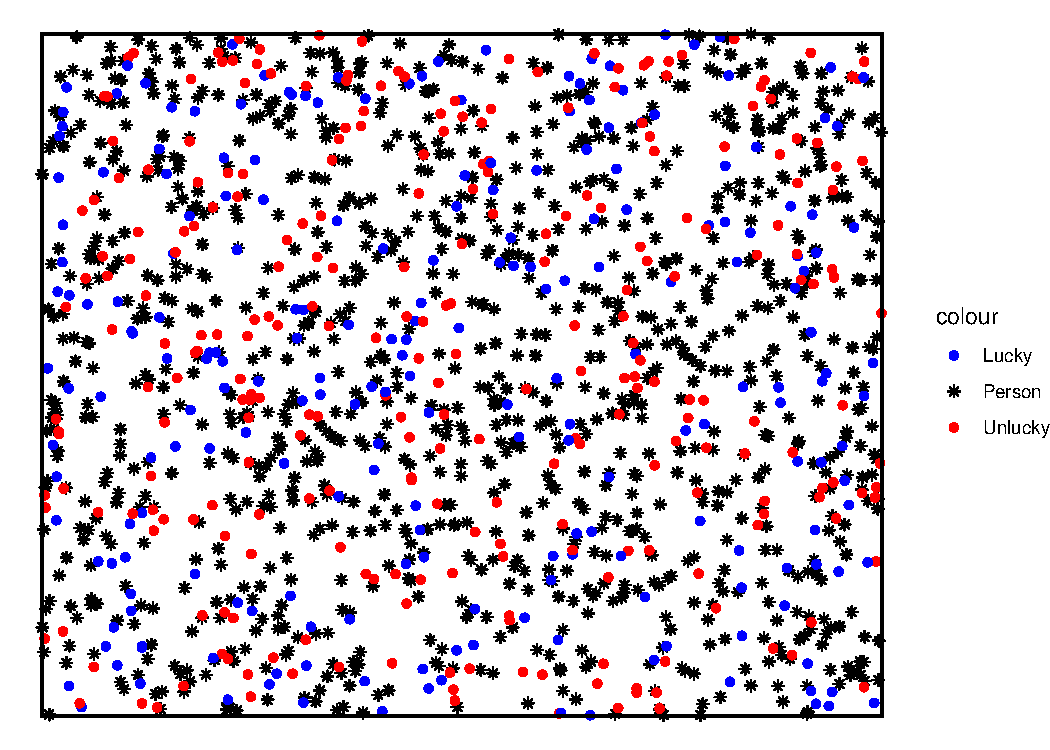
\includegraphics[width=\maxwidth]{figure/unnamed-chunk-4-1} 
\end{knitrout}

\caption{The beginning map of simulated people and lucky/unlucky events}
\label{plot1}
\end{center}
\end{figure}


%%%%%%%%%%%%%%%%%%%%%%%%%%%%%%%%%%%%%%%%%%%%%%%%%%%%%%%%%%%%%%%%%%%%%%%%%%%%%%%%
%%%%%%%%%%%%%%%%%%%%%%%%%%%%%%%%%%%%%%%%%%%%%%%%%%%%%%%%%%%%%%%%%%%%%%%%%%%%%%%%
% Question 4
%%%%%%%%%%%%%%%%%%%%%%%%%%%%%%%%%%%%%%%%%%%%%%%%%%%%%%%%%%%%%%%%%%%%%%%%%%%%%%%%
%%%%%%%%%%%%%%%%%%%%%%%%%%%%%%%%%%%%%%%%%%%%%%%%%%%%%%%%%%%%%%%%%%%%%%%%%%%%%%%%
\item Write a function called \texttt{move.event()} that takes the following arguments
\begin{align*}
\texttt{x} &= x~\textrm{coordinate}\\
\texttt{y} &= y~\textrm{coordinate}\\
\texttt{dist} &= \textrm{distance to move}
\end{align*}
and performs the following.
\begin{enumerate}
\item Pick a random angle $\theta$ between $0$ and $2\pi$ for the event to move.\\
\textbf{Hint:} Use the \texttt{runif()} function in \texttt{R}.
\item Compute the change in $x$ and $y$. Recall,
\begin{align*}
\Delta{x} = \texttt{dist} \times \cos(\theta)\\
\Delta{y} = \texttt{dist} \times \sin(\theta)
\end{align*}
\item Update the values of \texttt{x} and \texttt{y} in temporary objects \texttt{x.new} and \texttt{y.new}.
\item If the points have moved outside of the unit square, send them to the other side of the square. Note, you can update $x$ and $y$ as follows.
\begin{align*}
x = 
\begin{cases}
x   & x \in  [0, 1] \\
-x   & x \in  [-1, 0)\\
(2-x) & x \in  (1, 2] \\
\end{cases}
\end{align*}
\item Return the new location of the event.
\end{enumerate}

\begin{knitrout}\scriptsize
\definecolor{shadecolor}{rgb}{0.969, 0.969, 0.969}\color{fgcolor}\begin{kframe}
\begin{alltt}
\hldef{move.event} \hlkwb{<-} \hlkwa{function}\hldef{(}\hlkwc{x}\hldef{,} \hlkwc{y}\hldef{,} \hlkwc{dist}\hldef{)\{}

  \hlcom{#a}
  \hldef{theta} \hlkwb{=} \hlkwd{runif}\hldef{(}\hlkwc{n} \hldef{=} \hlnum{1}\hldef{,} \hlkwc{min} \hldef{=} \hlnum{0}\hldef{,} \hlkwc{max} \hldef{=} \hlnum{2}\hlopt{*}\hldef{pi)}

  \hlcom{#b}
  \hldef{delta.x} \hlkwb{=} \hldef{dist} \hlopt{*} \hlkwd{cos}\hldef{(theta)}
  \hldef{delta.y} \hlkwb{=} \hldef{dist} \hlopt{*} \hlkwd{sin}\hldef{(theta)}

  \hlcom{#c}
  \hldef{x.new} \hlkwb{=} \hldef{x} \hlopt{+} \hldef{delta.x}
  \hldef{y.new} \hlkwb{=} \hldef{y} \hlopt{+} \hldef{delta.y}

  \hlcom{#d}
  \hlkwa{if}\hldef{(x.new} \hlopt{< -}\hlnum{1}\hldef{)\{}
    \hldef{x.new} \hlkwb{=} \hlopt{-}\hlnum{1} \hlopt{*} \hldef{x.new}
  \hldef{\}} \hlkwa{else if} \hldef{(x.new} \hlopt{>} \hlnum{1}\hldef{)\{}
    \hldef{x.new} \hlkwb{=} \hlnum{2} \hlopt{-} \hldef{x.new}
  \hldef{\}}

  \hlkwa{if}\hldef{(y.new} \hlopt{< -}\hlnum{1}\hldef{)\{}
    \hldef{y.new} \hlkwb{=} \hlopt{-}\hlnum{1} \hlopt{*} \hldef{y.new}
  \hldef{\}} \hlkwa{else if} \hldef{(y.new} \hlopt{>} \hlnum{1}\hldef{)\{}
    \hldef{y.new} \hlkwb{=} \hlnum{2} \hlopt{-} \hldef{y.new}
  \hldef{\}}

  \hlkwd{return}\hldef{(}\hlkwd{c}\hldef{(x.new, y.new))}

\hldef{\}}
\end{alltt}
\end{kframe}
\end{knitrout}

%%%%%%%%%%%%%%%%%%%%%%%%%%%%%%%%%%%%%%%%%%%%%%%%%%%%%%%%%%%%%%%%%%%%%%%%%%%%%%%%
%%%%%%%%%%%%%%%%%%%%%%%%%%%%%%%%%%%%%%%%%%%%%%%%%%%%%%%%%%%%%%%%%%%%%%%%%%%%%%%%
% Question 5
%%%%%%%%%%%%%%%%%%%%%%%%%%%%%%%%%%%%%%%%%%%%%%%%%%%%%%%%%%%%%%%%%%%%%%%%%%%%%%%%
%%%%%%%%%%%%%%%%%%%%%%%%%%%%%%%%%%%%%%%%%%%%%%%%%%%%%%%%%%%%%%%%%%%%%%%%%%%%%%%%
\item Conduct the simulation over 80 six-month periods by conducting the following steps in a loop for each six-month period.
\begin{enumerate}
\item Check to see whether each person is within 1/201 of an event. This is the quantity used by \cite{Pluchino18} to determine when an event and a person interact.\\
\textbf{Hint:} This requires you to compute the distance from each person to each event. Recall, you can compute the distance between two points $(x_1, y_1)$ and $(x_2, y_2)$ as
\[\textrm{Distance} = \sqrt{(x_1-x_2)^2 + (y_1-y_2)^2}.\]
\item When a person is within 1/201 of a ``Unlucky" event, halve their \texttt{Capital} regardless of their \texttt{Talent}.
\item When a person is within 1/201 of a ``Lucky" event, and double their \texttt{Capital} if their \texttt{Talent} is greater than a randomly generated number between 0 and 1 using \texttt{runif()}. 
\item Update the location of events using the \texttt{move.event()} function with \texttt{dist=1/201}. 
\end{enumerate}
\textbf{Hint:} While it is not the \emph{only} way to complete this task, I used nested \texttt{for()} loops -- six-month time frames, people, events.\\
\textbf{Note:} Once you get it to work, set \texttt{eval=F} in your \texttt{R} chunk preamble. It takes a few minutes to complete and that will be annoying as you continue to compile your homework.\\


\begin{knitrout}\scriptsize
\definecolor{shadecolor}{rgb}{0.969, 0.969, 0.969}\color{fgcolor}\begin{kframe}
\begin{alltt}
\hlcom{# a}

\hldef{distance} \hlkwb{<-} \hlkwd{rep}\hldef{(}\hlnum{NA}\hldef{,} \hlnum{500}\hldef{)}

\hlkwa{for}\hldef{(i} \hlkwa{in} \hlnum{1}\hlopt{:}\hlnum{80}\hldef{)\{}
  \hlkwa{for} \hldef{(j} \hlkwa{in} \hlnum{1}\hlopt{:}\hlnum{1000}\hldef{)\{}
    \hlkwa{for}\hldef{(k} \hlkwa{in} \hlnum{1}\hlopt{:}\hlnum{500}\hldef{)\{}

      \hldef{distance[k]} \hlkwb{=} \hlkwd{sqrt}\hldef{((sim}\hlopt{$}\hldef{x[j]} \hlopt{-} \hldef{Events}\hlopt{$}\hldef{x[k])}\hlopt{^}\hlnum{2} \hlopt{+} \hldef{(sim}\hlopt{$}\hldef{y[j]} \hlopt{-} \hldef{Events}\hlopt{$}\hldef{y[k])}\hlopt{^}\hlnum{2}\hldef{)}

      \hlcom{#b}
      \hlkwa{if}\hldef{(distance[k]} \hlopt{<=} \hlnum{1}\hlopt{/}\hlnum{201}\hldef{)\{}

        \hlkwa{if}\hldef{(Events}\hlopt{$}\hldef{Type[k]} \hlopt{==} \hlsng{"Unlucky"}\hldef{)\{}

          \hldef{sim}\hlopt{$}\hldef{Capital[j]} \hlkwb{=} \hldef{sim}\hlopt{$}\hldef{Capital[j]} \hlopt{*} \hlnum{0.5}
          \hldef{sim}\hlopt{$}\hldef{Unlucky[j]} \hlkwb{=} \hldef{sim}\hlopt{$}\hldef{Unlucky[j]} \hlopt{+} \hlnum{1}

        \hlcom{#c}
        \hldef{\}}\hlkwa{else}\hldef{\{}

          \hldef{talent_check} \hlkwb{<-} \hlkwd{runif}\hldef{(}\hlkwc{n} \hldef{=} \hlnum{1}\hldef{,} \hlkwc{min} \hldef{=} \hlnum{0}\hldef{,} \hlkwc{max} \hldef{=} \hlnum{1}\hldef{)}

          \hlkwa{if}\hldef{(sim}\hlopt{$}\hldef{Talent[j]} \hlopt{>} \hldef{talent_check)\{}

            \hldef{sim}\hlopt{$}\hldef{Capital[j]} \hlkwb{=} \hldef{sim}\hlopt{$}\hldef{Capital[j]} \hlopt{*} \hlnum{2}
            \hldef{sim}\hlopt{$}\hldef{Lucky[j]} \hlkwb{=} \hldef{sim}\hlopt{$}\hldef{Lucky[j]} \hlopt{+} \hlnum{1}
          \hldef{\}}
        \hldef{\}}
      \hldef{\}}
    \hldef{\}}
  \hldef{\}}

  \hlcom{#d}
  \hlkwa{for}\hldef{(e} \hlkwa{in} \hlnum{1}\hlopt{:}\hlnum{500}\hldef{)\{}

    \hldef{new_location} \hlkwb{<-} \hlkwd{move.event}\hldef{(Events}\hlopt{$}\hldef{x[e], Events}\hlopt{$}\hldef{y[e],} \hlnum{1}\hlopt{/}\hlnum{201}\hldef{)}

    \hldef{Events}\hlopt{$}\hldef{x[e]} \hlkwb{<-} \hldef{new_location[}\hlnum{1}\hldef{]}

    \hldef{Events}\hlopt{$}\hldef{y[e]} \hlkwb{<-} \hldef{new_location[}\hlnum{2}\hldef{]}

  \hldef{\}}

\hldef{\}}
\end{alltt}
\end{kframe}
\end{knitrout}

%%%%%%%%%%%%%%%%%%%%%%%%%%%%%%%%%%%%%%%%%%%%%%%%%%%%%%%%%%%%%%%%%%%%%%%%%%%%%%%%
%%%%%%%%%%%%%%%%%%%%%%%%%%%%%%%%%%%%%%%%%%%%%%%%%%%%%%%%%%%%%%%%%%%%%%%%%%%%%%%%
% Question 6
%%%%%%%%%%%%%%%%%%%%%%%%%%%%%%%%%%%%%%%%%%%%%%%%%%%%%%%%%%%%%%%%%%%%%%%%%%%%%%%%
%%%%%%%%%%%%%%%%%%%%%%%%%%%%%%%%%%%%%%%%%%%%%%%%%%%%%%%%%%%%%%%%%%%%%%%%%%%%%%%%
\item Does Talent matter? For the following, use the \texttt{simulation.csv} to evaluate the results. Note that these data come from 100 runs of the simulation, where we saved the top 1\% of people according to their accumulated capital/success. Is the mean talent of those in the top 1\% different from the generating $\mu_T=0.60$?
\begin{enumerate}
\item Load the data into \texttt{R}.
\begin{knitrout}\scriptsize
\definecolor{shadecolor}{rgb}{0.969, 0.969, 0.969}\color{fgcolor}\begin{kframe}
\begin{alltt}
\hlcom{#a}
\hldef{results} \hlkwb{<-} \hlkwd{read.csv}\hldef{(}\hlsng{'simulation.csv'}\hldef{)}
\end{alltt}
\end{kframe}
\end{knitrout}
\item Compute a statistic or statistics and create a figure or figures that summarize the data and begin to answer the research question.


\begin{knitrout}\scriptsize
\definecolor{shadecolor}{rgb}{0.969, 0.969, 0.969}\color{fgcolor}\begin{kframe}
\begin{alltt}
\hlkwd{library}\hldef{(xtable)}
\hldef{one_percent_sum} \hlkwb{<-} \hlkwd{t.test}\hldef{(results}\hlopt{$}\hldef{Talent,} \hlkwc{mu} \hldef{=} \hlnum{0.6}\hldef{)}\hlopt{$}\hldef{conf.int}
\hldef{normal_sum} \hlkwb{<-} \hlkwd{t.test}\hldef{(sim}\hlopt{$}\hldef{Talent,} \hlkwc{mu} \hldef{=} \hlnum{0.6}\hldef{)}\hlopt{$}\hldef{conf.int}

\hldef{tab.sum} \hlkwb{<-} \hlkwd{data.frame}\hldef{(}\hlkwc{Group} \hldef{=} \hlkwd{c}\hldef{(}\hlsng{"One Percent"}\hldef{,} \hlsng{"Normal Simulation"}\hldef{),}
                      \hlkwc{Mean_Talent} \hldef{=} \hlkwd{c}\hldef{(}\hlkwd{mean}\hldef{(results}\hlopt{$}\hldef{Talent),}\hlkwd{mean}\hldef{(sim}\hlopt{$}\hldef{Talent)),}
                  \hlkwc{Lower_CI} \hldef{=} \hlkwd{c}\hldef{(one_percent_sum[}\hlnum{1}\hldef{], normal_sum[}\hlnum{1}\hldef{]),}
                  \hlkwc{Upper_CI} \hldef{=} \hlkwd{c}\hldef{(one_percent_sum[}\hlnum{2}\hldef{], normal_sum[}\hlnum{2}\hldef{]))}
\hldef{tab.sum} \hlkwb{<-}\hlkwd{xtable}\hldef{(tab.sum,}\hlkwc{label} \hldef{=} \hlsng{"tab.sum"}\hldef{,} \hlkwc{caption} \hldef{=} \hlsng{"Mean Talent and Confidence Intervals of Both Groups"}\hldef{)}
\end{alltt}
\end{kframe}
\end{knitrout}

\begin{kframe}
\begin{alltt}
\hlkwd{print}\hldef{(tab.sum,}
\hlkwc{table.placement} \hldef{=} \hlsng{"H"}\hldef{,} \hlkwc{include.rownames}\hldef{=}\hlnum{FALSE}\hldef{,} \hlkwc{size} \hldef{=} \hlsng{"small"}\hldef{)}
\end{alltt}
\end{kframe}% latex table generated in R 4.4.2 by xtable 1.8-4 package
% Sun Sep  7 16:01:18 2025
\begin{table}[H]
\centering
\begingroup\small
\begin{tabular}{lrrr}
  \hline
Group & Mean\_Talent & Lower\_CI & Upper\_CI \\ 
  \hline
One Percent & 0.65 & 0.65 & 0.66 \\ 
  Normal Simulation & 0.61 & 0.60 & 0.61 \\ 
   \hline
\end{tabular}
\endgroup
\caption{Mean Talent and Confidence Intervals of Both Groups} 
\label{tab.sum}
\end{table}



\begin{figure}[H]
\begin{center}

\begin{knitrout}\scriptsize
\definecolor{shadecolor}{rgb}{0.969, 0.969, 0.969}\color{fgcolor}\begin{kframe}
\begin{alltt}
\hlkwd{ggplot}\hldef{(}\hlkwc{data} \hldef{= tab.sum,} \hlkwd{aes}\hldef{(}\hlkwc{x} \hldef{= Group,} \hlkwc{y} \hldef{= Mean_Talent))} \hlopt{+}
  \hlkwd{geom_col}\hldef{()} \hlopt{+}
  \hlkwd{geom_errorbar}\hldef{(}\hlkwd{aes}\hldef{(}\hlkwc{ymin} \hldef{= Lower_CI,} \hlkwc{ymax} \hldef{= Upper_CI),} \hlkwc{width} \hldef{=} \hlnum{0.25}\hldef{)} \hlopt{+}
  \hlkwd{theme_bw}\hldef{()} \hlopt{+}
  \hlkwd{geom_hline}\hldef{(}\hlkwc{yintercept} \hldef{=} \hlnum{0}\hldef{)} \hlopt{+}
  \hlkwd{labs}\hldef{(}\hlkwc{x} \hldef{=} \hlsng{""}\hldef{,}
       \hlkwc{y} \hldef{=} \hlsng{"Mean Talent"}\hldef{,}
       \hlkwc{title} \hldef{=} \hlsng{"Comparing Talent: 1% vs. Normal Simulation"}\hldef{)} \hlopt{+}
  \hlkwd{ylim}\hldef{(}\hlnum{0}\hldef{,}\hlnum{1}\hldef{)}
\end{alltt}
\end{kframe}

\includegraphics[width=\maxwidth]{figure/unnamed-chunk-10-1} 
\end{knitrout}

\caption{Comparison Barplots of Talent}
\label{plot2}
\end{center}
\end{figure}

\begin{figure}[H]
\begin{center}


\begin{knitrout}\scriptsize
\definecolor{shadecolor}{rgb}{0.969, 0.969, 0.969}\color{fgcolor}\begin{kframe}
\begin{alltt}
\hlkwd{ggplot}\hldef{(}\hlkwc{data} \hldef{= sim,} \hlkwd{aes}\hldef{(}\hlkwc{x} \hldef{= Talent,} \hlkwc{y} \hldef{=} \hlkwd{log}\hldef{(Capital)))} \hlopt{+}
  \hlkwd{geom_point}\hldef{()} \hlopt{+}
  \hlkwd{geom_smooth}\hldef{(}\hlkwd{aes}\hldef{(}\hlkwc{color} \hldef{=} \hlsng{"Best-Fit Model"}\hldef{))} \hlopt{+}
  \hlkwd{theme_bw}\hldef{()} \hlopt{+}
  \hlkwd{ggtitle}\hldef{(}\hlsng{'Talent vs. log(Capital)'}\hldef{)} \hlopt{+}
  \hlkwd{labs}\hldef{(}\hlkwc{subtitle} \hldef{=} \hlkwd{paste}\hldef{(}\hlsng{'r ='}\hldef{,} \hlkwd{round}\hldef{(}\hlkwd{cor}\hldef{(sim}\hlopt{$}\hldef{Talent, sim}\hlopt{$}\hldef{Capital),} \hlnum{3}\hldef{)))} \hlopt{+}
  \hlkwd{theme}\hldef{(}\hlkwc{legend.title} \hldef{=} \hlkwd{element_blank}\hldef{())}
\end{alltt}
\end{kframe}
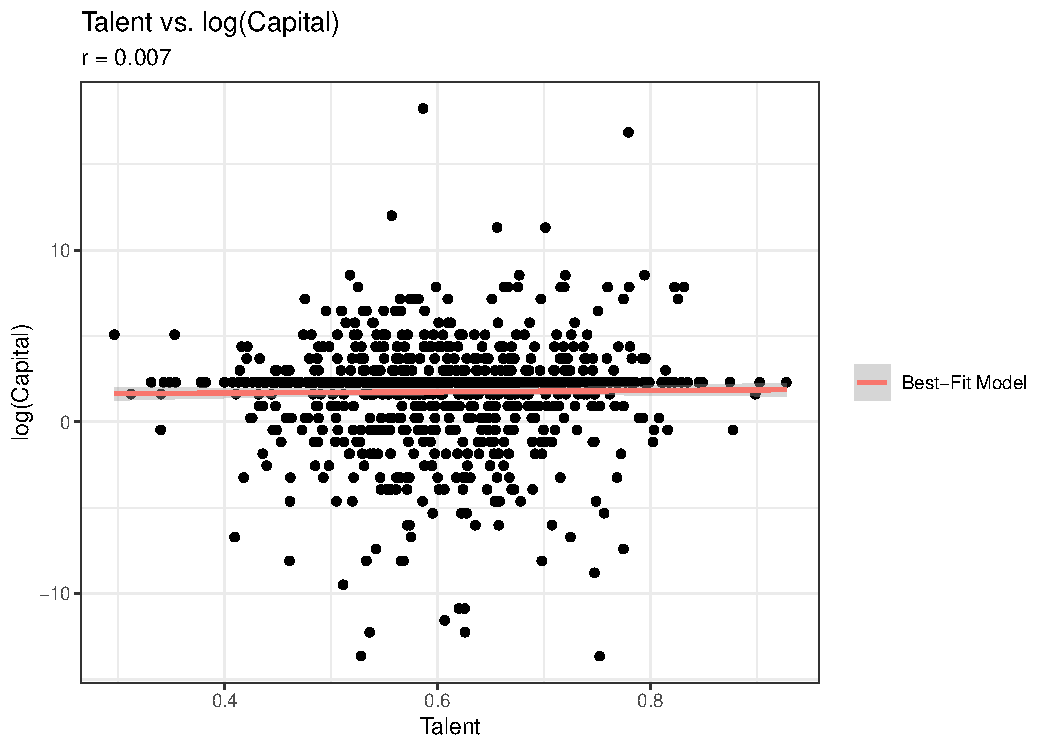
\includegraphics[width=\maxwidth]{figure/unnamed-chunk-11-1} 
\end{knitrout}

\caption{Scatter Plot of Talent against log(Capital)}
\label{plot3}
\end{center}
\end{figure}

\item Evaluate whether the conditions for using a $t$-based inference.
\begin{knitrout}\scriptsize
\definecolor{shadecolor}{rgb}{0.969, 0.969, 0.969}\color{fgcolor}\begin{kframe}
\begin{alltt}
\hlcom{#c}
\hlkwd{library}\hldef{(stats)}
\hlkwd{shapiro.test}\hldef{(results}\hlopt{$}\hldef{Talent)}
\end{alltt}
\begin{verbatim}
## 
## 	Shapiro-Wilk normality test
## 
## data:  results$Talent
## W = 0.99908, p-value = 0.9114
\end{verbatim}
\end{kframe}
\end{knitrout}
\item Regardless of your answer in part (b), conduct a $t$-test.
\begin{knitrout}\scriptsize
\definecolor{shadecolor}{rgb}{0.969, 0.969, 0.969}\color{fgcolor}\begin{kframe}
\begin{alltt}
\hlcom{#d}
\hlkwd{t.test}\hldef{(results}\hlopt{$}\hldef{Talent,} \hlkwc{mu} \hldef{=} \hlnum{0.6}\hldef{)}
\end{alltt}
\begin{verbatim}
## 
## 	One Sample t-test
## 
## data:  results$Talent
## t = 17.168, df = 999, p-value < 2.2e-16
## alternative hypothesis: true mean is not equal to 0.6
## 95 percent confidence interval:
##  0.6462244 0.6581555
## sample estimates:
## mean of x 
##   0.65219
\end{verbatim}
\end{kframe}
\end{knitrout}
\item Regardless of your answer in part (b), compute a $t$-interval.
\begin{knitrout}\scriptsize
\definecolor{shadecolor}{rgb}{0.969, 0.969, 0.969}\color{fgcolor}\begin{kframe}
\begin{alltt}
\hlcom{#e}
\hlkwd{t.test}\hldef{(results}\hlopt{$}\hldef{Talent,} \hlkwc{mu} \hldef{=} \hlnum{0.6}\hldef{)}\hlopt{$}\hldef{conf.int}
\end{alltt}
\begin{verbatim}
## [1] 0.6462244 0.6581555
## attr(,"conf.level")
## [1] 0.95
\end{verbatim}
\end{kframe}
\end{knitrout}
\item Write an interpretation of your work above and provide a preliminary answer to the research
question.
\begin{knitrout}\scriptsize
\definecolor{shadecolor}{rgb}{0.969, 0.969, 0.969}\color{fgcolor}\begin{kframe}
\begin{alltt}
\hlkwd{library}\hldef{(effectsize)}
\hlkwd{hedges_g}\hldef{(results}\hlopt{$}\hldef{Talent,} \hlkwc{mu} \hldef{=} \hlnum{0.6}\hldef{)}
\end{alltt}
\begin{verbatim}
## Hedges' g |       95% CI
## ------------------------
## 0.54      | [0.48, 0.61]
## 
## - Deviation from a difference of 0.6.
\end{verbatim}
\begin{alltt}
\hlkwd{interpret_hedges_g}\hldef{(}\hlnum{0.54}\hldef{)}
\end{alltt}
\begin{verbatim}
## [1] "medium"
## (Rules: cohen1988)
\end{verbatim}
\end{kframe}
\end{knitrout}


\end{enumerate}
\textbf{Note:} For this question, provide a solution under each part.

After taking the top one percent of participants in capital after one hundred simulations, a precursory look at the mean talent of the one percent compared to a run of the normal simulation, we see a discernible but relatively smell visual difference. As shown in Figure:  \ref{plot2}, mean talent is plotted with error bars representing a 95 percent confidence interval, visually showing the data provided in Figure: \ref{tab.sum}. 

The especially sensitive Shapiro-Wilkes test for normality gives us a test statistic W of 0.9908 and p = 0.9114, giving assurance that the talent measures from the top one percent are normally distributed for the t-test. 

A t-test was conducted on the talent measures from the one-percent to see if the true mean of the talent measures was different than the overall average given of 0.6. The test statistic from our two sided test was t = 17.168 and p \textless 0.0001. A 95 percent confidence interval of the talent measures is given: [0.646, 0.658]. Because the p-value given is less than our given alpha of 0.05, we have strong evidence that the true value of talent of the top 1 percent of individuals regarding capital is not equal to 0.6. The effect size measure hedge's g gives an effect size of 0.54 with a 95 percent confidence interval of [0.48, 0.61], indicating a moderate deviation from the null. 

Our hypothesis test would lead us to believe that those who gain the most capital are significantly more talented than the average person. However, as shown in Figure: \ref{plot2}, the difference between the average talent from the top one percent and the normal pool of individuals is only slightly higher on visual analysis, plus, as seen in Figure: \ref{plot3}, in a single run of the simulation, the correlation between talent and capital is essentially non-existent. This leads us to the conclusion that while talent is a factor in gaining capital after repeated testing and thousands of individuals, in a single simulation, the effect of talent on capital is much less convincing, suggesting that other factors are very, if not more, important. 

%%%%%%%%%%%%%%%%%%%%%%%%%%%%%%%%%%%%%%%%%%%%%%%%%%%%%%%%%%%%%%%%%%%%%%%%%%%%%%%%
%%%%%%%%%%%%%%%%%%%%%%%%%%%%%%%%%%%%%%%%%%%%%%%%%%%%%%%%%%%%%%%%%%%%%%%%%%%%%%%%
% Optional Practice
%%%%%%%%%%%%%%%%%%%%%%%%%%%%%%%%%%%%%%%%%%%%%%%%%%%%%%%%%%%%%%%%%%%%%%%%%%%%%%%%
%%%%%%%%%%%%%%%%%%%%%%%%%%%%%%%%%%%%%%%%%%%%%%%%%%%%%%%%%%%%%%%%%%%%%%%%%%%%%%%%
\item \textbf{(Optional)} Attempt to recreate some of the other plots from \cite{Pluchino18}. Based on the simulation, you can recreate Figures 2-6 using your simulation. You can recreate Figures 7-9 using the \texttt{simulation.csv} file.
\item \textbf{(Optional)} I, personally, wonder whether the ``success'' or ending capital depended on how close individuals were to lucky events at the beginning of the simulation. That is, instead of considering ``luck" as whether a lucky event crossed an individual we considered starting luck. Compute a statistic and create a figure that helps answer this question.
\item \textbf{(Optional)} You may or may not have been completely satisfied when you evaluated the conditions for using a $t$-test. Conduct a bootstrap test and/or a randomization test. Does the research answer change?
\item \textbf{(Optional)} One possible extension to their work is to consider how bias plays a role. For example, \cite{Eames24} showed that there was bias in the evaluation of applications based on whether applicants listed pronouns, and, if they did, what their pronouns were. \cite{Gaddis21} show that there continues to be racial and ethnic discrimination in hiring. And, interestingly, these racial biases can be exacerbated by withholding certain information \citep[e.g., ban the box initiatives; see][]{Agan18}.\\

To investigate this, we made the following adjustments to the simulation:
\begin{itemize}
\item Our \texttt{People tibble} contained 2000 individuals -- 1000 ``disadvantaged" and 1000 ``advantaged" individuals.
\item We created a \texttt{talent.differential} object meant to describe how individuals were \emph{perceived} and we use perceived talent to determine whether we double a person's capital when a lucky event crosses their path. For this homework, consider the following setup,
\begin{align*}
\texttt{talent.differential} &= 0.30 \\
\texttt{perceived.talent}   &= \texttt{Talent} \pm \texttt{talent.differential/2}
\end{align*}
where we add for the advantaged group and subtract for the disadvantaged group.
\end{itemize}

In the end, we can see whether the disparity in \emph{perceived} talent of this new simulation affects the results. Researchers believe that this situation may yield more mediocre advantaged people in the most successful group.\\

For the following questions, use the \texttt{bias-simulation.csv} to evaluate the results. Note that these data come from 100 runs of the simulation, where we saved the top 1\% of people according to their accumulated capital/success. We want to directly compare the advantaged and disadvantaged groups.
\begin{enumerate}
\item Compute a statistic or statistics and create a figure or figures that summarize the data and begin to answer the research question.
\item Use the documentation from calling \texttt{?t.test} to perform a two-sample test that directly compares the groups. Also compute the two-sample confidence interval.
\item Write an interpretation of your work above and provide a preliminary answer to the research question. 
\end{enumerate}
\end{enumerate}
\bibliography{bib}
\end{document}
